\scanpage{70}
% archive sheet number: 69

\unsure{\deleted{l}a|\deleted{a}l}llant de la catégorie des schémas propres et lisses sur $k$ vers les F-cristaux gardués, \deleted{compatibles} qui est additif (pour la somme des $X$ ) et compatible avec $\otimes$ \inserted{\handwritten{une fois tensorisé par $\unsure{\mathbb{Q}|Q}_p$}} (le $\otimes$ des schémas étant le produit cartésien) de façon compatible ave\unsure{\deleted{v}c|\deleted{c}v} les associativités et commutativités (tant pour la somme que pour le produit), en faisant attention d'utiliser la règle de Koko pour la contrainte de commutativité. De plus, modulo des vérifications qui n'ont pas encore été faites par Berthelot, mais qui ne peuvent manquer de sortir prochainement, le foncteur précédent est même défini en prenant comme morphismes des correspondances algébriques à équivalence\handwritten{\begin{tikzpicture}[x=1cm,y=1cm,baseline=0cm]\draw[gray,thin] (0,.4).. controls (.25,.05) and (.3,-.25)..(.2,-.5);\end{tikzpicture}} algébrique près, et s'en va vers les F-cristaux \uline{non dégénér\unsure{\deleted{a}é|\deleted{é}a}s}; de façon précise, il doit être\handwritten{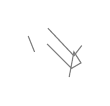
\begin{tikzpicture}[x=1cm,y=1cm,baseline=0cm]\draw[gray,thin] (-.4,.22)--(-.32,.02);\draw[gray,thin] (-.15,.32)--(.18,-.03)--(.28,.1);\draw[gray,thin] (-.16,.12)--(.15,-.19)--(.27,-.12)--(.18,.02)--(.12,-.3);\end{tikzpicture}} vrai que pour tout $i$, il existe un $V_i$ :\deleted{dans} $H^i\handwritten{\longrightarrow (}H^i\handwritten{)^{\unsure{\deleted{\sigma}\sigma|\sigma}}}$ tel que $F\ V_i=p^i\ \mathrm{id}$ , $V_iF=p^i\ \unsure{\deleted{\mathrm{u}}\mathrm{i}|\deleted{\mathrm{i}}\mathrm{u}|\mathrm{i}}\mathrm{d}$ (C'est en tous cas vrai si $X$ se remonte en car. 0) Modulo cette vérification, on trouve donc un foncteur
\[
H^{\handwritten{*}}_{\mathrm{cris}}\substack{\deleted{\unsure{\mathbb{W}|W}}\\\handwritten{\unsure{\otimes|\deleted{K}|\deleted{W}}\mathbb{Q}_p}}:\text{schémas propres lisses sur }k\handwritten{\longrightarrow \mathrm{Gr}\unsure{a|d}\mathrm{d}\unsure{\breve{f}}(}\mathrm{F}\unsure{\mathbb{C}|\mathrm{C}|\mathrm{c}|\mathrm{e}}\mathrm{riso}^{\handwritten{+}}(k)\handwritten{)}\ ,
\]
\handwritten{\begin{tikzpicture}[x=1cm,y=1cm,baseline=0cm]\draw[gray,thin] (0,-.35).. controls (.1,-.1) and (.18,.1)..(.16,.4);\end{tikzpicture}}compatible à\deleted{,} tout (un ``foncteur cohomologi\unsure{\deleted{q}e|\deleted{e}q}\deleted{ue}'' dans la terminologie de l'exposé de Kleiman \handwritten{[\quad]}). Bien entendu, on a $H^{\handwritten{2}}_{\mathrm{cris}}(P^1)=\mathbb{W}(-1)$ , plus généralement on devra avoir (quand Berthelot aura bien travaill\unsure{é|e}
\[
H^{2d\deleted{\unsure{*|i}}}_{\mathrm{cris}}(X)\handwritten{\simeq}\mathbb{W}(-d)
\]
si $X$ est géométriquement connexe et de dimension $d$, (isomorphisme canonique, compatible à la multiplication ...). En admettant le yoga des motifs (on a besoin ici de la structure graduée de la catégorie des motifs sur $k$, pour pouvoir canuler par la règle de Koko la contrainte de commutativité naturelle sur les motifs, provenant de l'isomorphisme de commutativité $X\mathrm{x}Y\handwritten{\simeq}Y\mathrm{x}X$ sur les schémas ...) on aura un homomorphisme de gerbes canonique
\[
\handwritten{\unsure{\Pi|\deleted{\Pi}\Pi}}(k)_{\handwritten{\mathbb{Q}_p}}\handwritten{\longleftarrow}\underline{G}(k)\ ,\qquad
\handwritten{\text{associé \unsure{au|àu} }\inserted{\text{$\otimes$-foncteur}}\mathrm{Mot}(k)\longrightarrow\mathrm{Fcriso}(k)}
\]
où $\handwritten{\Pi}(k)$ e\unsure{\deleted{z}s|\deleted{s}z}t la gerbe associée à la catégorie tannakienne (sur $\underline{Q}$)
